%%%%%%%%%%%%%%%%%%%%%%%%%%%%%%%%%%%%%%%%%%%%%%%%%%%%%%%%%%%%%%%%%%%%%%%%%%%%%%%
\section{Flux Separability Approximation}
\label{sec:flux-separability}
%%%%%%%%%%%%%%%%%%%%%%%%%%%%%%%%%%%%%%%%%%%%%%%%%%%%%%%%%%%%%%%%%%%%%%%%%%%%%%%

The steady-state Boltzmann transport equation is integro-differential in the neutron angular flux $\psi(\mathbf{r},\mathbf{\Omega},E)$ and balances the rate of change of the population of neutrons in phase space to the difference between the production and loss rates of neutrons within a closed system,

\begin{dmath}
\label{eqn:transport-eqn-ce}
\mathbf{\Omega} \cdot \nabla \psi(\mathbf{r},\mathbf{\Omega},E) + \Sigma_{t}(\mathbf{r},E)\psi(\mathbf{r},\mathbf{\Omega},E) = Q(\mathbf{r},\mathbf{\Omega},E)
\end{dmath}

%\int\displaylimits_{0}^{\infty}\int\displaylimits_{4\pi} \Sigma_{s}(\mathbf{r},{\mathbf{\Omega'}\rightarrow\mathbf{\Omega}},{E'\rightarrow E}) \psi(\mathbf{r},\mathbf{\Omega'},E') \mathrm{d}\mathbf{\Omega'} \mathrm{d}E' + \frac{1}{4\pi k_{eff}}\int\displaylimits_{0}^{\infty}\int\displaylimits_{4\pi} \nu\Sigma_{f}(\mathbf{r},{E'\rightarrow E})\psi(\mathbf{r},\mathbf{\Omega'},E') \mathrm{d}\mathbf{\Omega'} \mathrm{d}E'

\noindent where $Q(\mathbf{r},\mathbf{\Omega},E)$ is the source of neutrons from scattering, fission production or external sources.

Monte Carlo methods typically employ a continuous energy representation for the spatial $\mathbf{r}$, angle $\mathbf{\Omega}$ and energy $E$ variables. Deterministic methods apply some form of discretization to each of these variables. For example, the multi-group approach subdivides the neutron's energy into discrete bins known as energy groups $g$ which are indexed starting at 1 for high energies and ending with $G$ for low energies,

\begin{dmath}
\label{eqn:transport-eqn-mg}
\mathbf{\Omega} \cdot \nabla \psi_{g}(\mathbf{r},\mathbf{\Omega}) + \Sigma_{t,g}(\mathbf{r},\mathbf{\Omega})\psi_{g}(\mathbf{r},\mathbf{\Omega}) = Q_{g}(\mathbf{r},\mathbf{\Omega})
\end{dmath}

\noindent where the group-wise angular flux $\psi_{g}(\mathbf{r},\mathbf{\Omega})$ and source $Q_{g}(\mathbf{r},\mathbf{\Omega})$ are integrated across each energy group $g$:

\begin{dmath}
\label{eqn:groupwise-flux}
\psi_{g}(\mathbf{r},\mathbf{\Omega}) = \int\displaylimits_{E_{g}}^{E_{g-1}} \psi(\mathbf{r},\mathbf{\Omega},E)\mathrm{d}E
\end{dmath}

\begin{dmath}
\label{eqn:groupwise-source}
Q_{g}(\mathbf{r},\mathbf{\Omega}) = \int\displaylimits_{E_{g}}^{E_{g-1}} Q(\mathbf{r},\mathbf{\Omega},E)\mathrm{d}E
\end{dmath}

%\frac{1}{4\pi}\sum_{g'=1}^{G} \Sigma_{s,g' \rightarrow g}(\mathbf{r}) \phi_{g'}(\mathbf{r}) + \frac{1}{4\pi k_{eff}}\sum_{g'=1}^{G} \nu\Sigma_{f,g' \rightarrow g}(\mathbf{r})\phi_{g'}(\mathbf{r})

Equivalence between Eqns.~\ref{eqn:transport-eqn-ce} and~\ref{eqn:transport-eqn-mg} will be maintained if the $\Sigma_{t,g}(\mathbf{r},\mathbf{\Omega})$ is collapsed using the angular neutron flux,

\begin{dmath}
\label{eqn:sigt-mg}
\Sigma_{t,g}(\mathbf{r},\mathbf{\Omega}) \equiv \frac{\int\displaylimits_{E_{g}}^{E_{g-1}} \Sigma_{t}(\mathbf{r},E)\psi(\mathbf{r},\mathbf{\Omega},E)\mathrm{d}E}{\int\displaylimits_{E_{g}}^{E_{g-1}} \psi(\mathbf{r},\mathbf{\Omega},E)}
\end{dmath}

\noindent using a weighted average to preserve reaction rates in each energy group. This expression for $\Sigma_{t,g}(\mathbf{r},\mathbf{\Omega})$ presents a complication since it is dependent on the unknown angular flux.

The angular dependence of the total cross section is often treated with the flux separability approximation. Flux separability makes the simplifying assumption that the energy and angular dependence of the flux varies independently such that the angular flux can be written as the product of the scalar neutron flux $\phi(\mathbf{r},E)$ and some function $W(\mathbf{r}, \mathbf{\Omega})$:

\begin{dmath}
\label{eqn:flux-separate}
\psi(\mathbf{r},\mathbf{\Omega},E) \approx \phi(\mathbf{r},E) W(\mathbf{r},\mathbf{\Omega})
\end{dmath}

\noindent The angular dependence of the $\Sigma_{t,g}$ may then be eliminated by inserting Eqn.~\ref{eqn:flux-separate} into Eqn.~\ref{eqn:sigt-mg}, factoring out $W(\mathbf{r},\mathbf{\Omega})$ and writing $\Sigma_{t}$ in terms of the scalar flux,

\begin{dmath}
\label{eqn:sigt-mg-scalar}
\Sigma_{t,g}(\mathbf{r}) \approx \frac{\int\displaylimits_{E_{g}}^{E_{g-1}} \Sigma_{t}(\mathbf{r},E)\phi(\mathbf{r},E)W(\mathbf{r},\mathbf{\Omega})\mathrm{d}E}{\int\displaylimits_{E_{g}}^{E_{g-1}} \phi(\mathbf{r},E)W(\mathbf{r},\mathbf{\Omega})} = \frac{\int\displaylimits_{E_{g}}^{E_{g-1}} \Sigma_{t}(\mathbf{r},E)\phi(\mathbf{r},E)\mathrm{d}E}{\int\displaylimits_{E_{g}}^{E_{g-1}} \phi(\mathbf{r},E)}
\end{dmath}

\noindent The angular-independent total multi-group cross section is substituted into Eqn.~\ref{eqn:transport-eqn-mg} to derive the equation solved by most transport codes:

\begin{dmath}
\label{eqn:transport-eqn-mg-separate}
\mathbf{\Omega} \cdot \nabla \psi_{g}(\mathbf{r},\mathbf{\Omega}) + \Sigma_{t,g}(\mathbf{r})\psi_{g}(\mathbf{r},\mathbf{\Omega}) = Q_{g}(\mathbf{r},\mathbf{\Omega})
\end{dmath}

Although flux separability is a simple and commonly used approach to reduce the complexity of the multi-group total cross section, it is not always valid and may not preserve neutron balance. The flux separability approximation will necessarily hold in infinite homogeneous media since the flux does not vary in angle or space. However, the flux may vary greatly by angle in a heterogeneous geometry with significant spatial self-shielding.

For example, consider the flux from two different directions impinged upon a discretized spatial zone for one radial ring and angular sector in an LWR fuel pin in~\autoref{fig:incoming-outgoing}. The epithermal flux entering from the moderator will be unshielded and will likely be quite similar to the $\nicefrac{1}{E}$ asymptotic spectrum. In contrast, the flux which traverses the fuel pin will be significantly depressed in the resonant groups. As a result, the reaction rates for the incoming flux will be greater than those for the outgoing flux in resonant groups, which would be reflected in angular-dependent total MGXS.

This effect is illustrated in~\autoref{fig:batman-plots}, where a reference ultra-fine angular flux was used to collapse a single resonant cross section {\color{red}[with a peak/width of ?]}. The angular-dependent MGXS is shown separately for two discretized spatial zones at different radial and azimuthal locations and shaded in dark grey within the fuel pin. The cross section in the region at the fuel/moderator interface in~\autoref{fig:batman-plots-a} ranges from less than 5 to more than 50 barns for angles entering and leaving the fuel pin. The peaks near 60$^{\circ}$ and 120$^{\circ}$ are due to extra moderation experienced by neutrons streaming through the infinite rectilinear fuel pin lattice at those angles. The cross section in an interior of the fuel pin, such as the one shown in~\autoref{fig:batman-plots-b}, exhibits similar but less prominent properties since the flux is shielded in all directions.

\begin{figure}[ht!]
  \centering
  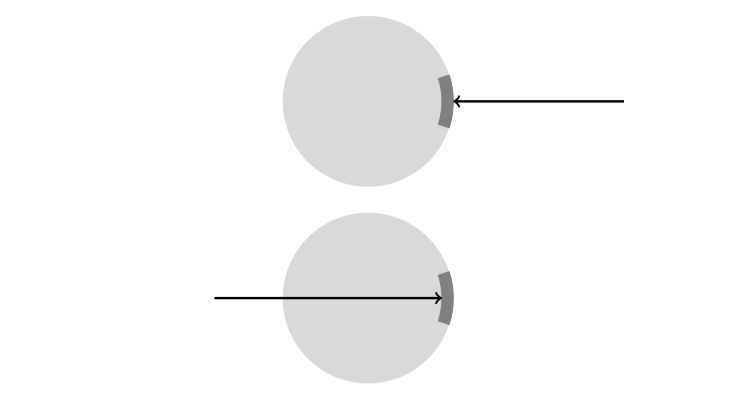
\includegraphics[width=\linewidth]{figures/incoming-outgoing}
  \caption{Angular flux impinged on an FSR from the moderator (top) and after traversing the fuel (bottom) \citep{gibson2016thesis}.}
\label{fig:incoming-outgoing}
\end{figure}

\begin{figure}[hb!]
\begin{subfigure}{.45\textwidth}
  \centering
  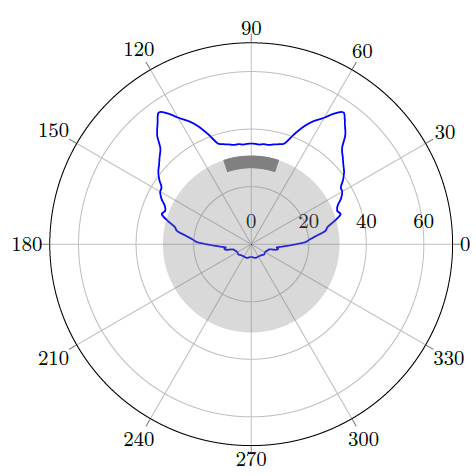
\includegraphics[width=0.8\linewidth]{figures/batman-1}
  \caption{}
  \label{fig:batman-plots-a}
\end{subfigure}
\begin{subfigure}{.45\textwidth}
  \centering
  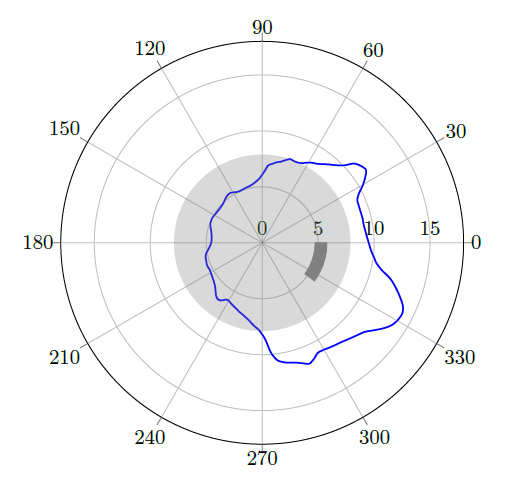
\includegraphics[width=0.8\linewidth]{figures/batman-2}
  \caption{}
  \label{fig:batman-plots-b}
\end{subfigure}
\caption{Angular-dependent capture MGXS for the 6.67 eV resonance group as a function of azimuthal angle for two different FSRs \citep{gibson2016thesis}. The radial axis is given in units of barns and the azimuthal axis in units of degrees.}
\label{fig:batman-plots}
\end{figure}

The variation of the total cross section in angle is typically neglected by deterministic transport codes which employ an isotropic multi-group total cross section $\Sigma_{t}(\mathbf{r})$ representation. To the authors' knowledge, the bias induced by the flux separability approximation on group-wise reaction rates and the eigenvalue is not well studied in the literature. This work seeks to address this by isolating and quantifying the impact of the flux separability approximation for PWR problems.